\subsection{Mass Transport In The Vadose Zone}\label{sec:transport}

To begin deriving a governing equation for contaminant transport in our VI scenario, we consider the continuity equation which states that the change of concentration in some volume of space depends on the advective and diffusive fluxes in and out of the system, as well as any generation or consumption inside the system.
\begin{equation}
  \frac{\partial c}{\partial t} + \nabla \cdot(j_\mathrm{adv} + j_\mathrm{diff}) - G = 0
\end{equation}
here $c$ [\si{\mol\per\metre\cubed}] is the concentration of the chemical species;
$t$ [\si{\second}] is time;
$j_\mathrm{adv}$ and $j_\mathrm{diff}$ [\si{\mol\per\second\per\metre\squared}] are the advective and diffusive fluxes respectively;
and $G$ [\si{\mol\per\second}] is the generation or consumption of the chemical species.\par

In our model we will assume that $G = 0$ as the groundwater is the sole contaminant source, i.e. there are no other sources of TCE in the soil, and TCE also does not readily degrade in soils\footnote{
Although, it is possible to introduce certain bacteria to bioremediate TCE in soils, but this typically requires specific conditions, which generally are not naturally met. Under these specific conditions TCE may be biodegraded by some bacteria\cite{fan_biodegradation_1993,little_trichloroethylene_1988}
}.
However, this term should be retained and an appropriate expression developed if one wants to model:
\begin{itemize}
  \item Biodegradation of some compound in the soil.
  \item Radon intrusion (remember radon gas is generated throughout soils and rocks).
  \item A soil or subsurface source, e.g. a leaky tank or evaporation from a liquid contaminant spill.
\end{itemize}\par

The advective flux is given by
\begin{equation}
  j_\mathrm{adv} = \vec{u} c
\end{equation}
where $\vec{u}$ [\si{\metre\per\second}] is a velocity vector.
The diffusive flux is given by Fick's Law
\begin{equation}
  j_\mathrm{diff} = -D \nabla c
\end{equation}
where $D$ [\si{\metre\squared\per\second}] is the diffusion coefficient of the contaminant in the soil air;
and $\nabla c$ [\si{\mol\per\metre\cubed\per\metre}] is a concentration gradient.
Thus we get the advection-diffusion equation which generally governs transport of a chemical species
\begin{equation}\label{eq:adv_diff}
  \frac{\partial c}{\partial t} + \nabla \cdot(\vec{u} c + -D \nabla c) = 0
\end{equation}
However, this simple gas phase transport equation will not accurately represent contaminant transport in the vadose zone if:
\begin{itemize}
  \item Contaminant transport occurs inside a variably saturated porous matrix which significantly affect transport properties.
  \item The contaminant concentration in the vadose zone is distributed between three phases - gas, water, and solid (via sorption).
\end{itemize}\par

The total contaminant concentration in the soil is given by the sum of the gas, water, and solid phase concentrations at any given point in the soil.
\begin{equation}
  c_T = \theta_w c_w + \theta_g c_g + c_s \rho_b
\end{equation}
Here $\theta_g$ and $\theta_w$ are the gas-filled and water-filled porosities respectively;
$c_T$ [\si{\mol\per\metre\cubed}] is the total soil contaminant concentration;
$c_w$ and $c_g$ [\si{\mol\per\metre\cubed}] are the contaminant concentrations in water and gas respectively;
$c_s$ [\si{\mol\per\kilogram}] is the solid phase or sorbed concentration per mass of soil;
and $\rho_b = (1-\theta_t) \rho$ [\si{\kilogram\per\metre\cubed}] is the bulk density of the soil, which can be calculated from the soil porosity $\theta_t$ and solid phase density of the soil $\rho$ [\si{\kilogram\per\metre\cubed}].\par

The attentive reader will now notice that \eqref{eq:adv_diff} depends on three variables instead of one.
However, remember that we're concerned with low contaminant concentrations, we can relate the gas and liquid phase concentrations via Henry's Law \eqref{eq:henrys_law}
\begin{equation}\label{eq:henrys_law}
  c_g = K_H c_w
\end{equation}
where, for example $K_H = 0.402$ is the dimensionless Henry's Law constant for TCE at \SI{20}{\degreeCelsius}\cite{heron_henrys_1998}.
We also assume that there are no temperature gradients throughout the vadose zone.\par

The solid phase concentration can be related to the others via a linear sorption isotherm.
Here either the gas-solid or water-solid sorption interaction can be chosen; the former is used in Chapter \ref{chp:sorption} where we will explore the effects of gas-solid sorption.
\begin{equation}
  c_s = \begin{cases}
    K_p c_w & \text{Water-solid sorption} \\
    K_p c_g = K_p K_H c_w & \text{Gas-solid sorption}
\end{cases}
\end{equation}
here $K_p$ [\si{\metre\cubed\per\kilogram}] is a sorption partitioning coefficient.\par

Another approach is to simply ignore the role of sorption completely, i.e. $K_p = 0$, which has historically been done in VI modeling and is done in the following parts of this example too.
The reason for this is two-fold.
\begin{enumerate}
  \item Relevant soil sorption data have not been readily available.
  \item At steady-state, sorption doesn't affect the solution; the fact that there is TCE sorbed to soil particles does not influence the vapor transport at steady state, since equilibrium is assumed to have been established prior to the steady-state analysis. This has been a common assumptions in most VI modeling studies, which have mostly focused on steady-state.
\end{enumerate}
Regardless, we will continue carrying the sorption $K_p$ term, because this will become relevant in Chapter \ref{chp:sorption} where experimentally derived relevant sorption data are available, and in which the role of this sorption process is considered in the context of transient models.\par

Using Henry's Law and the linear sorption assumptions we can relate the total contaminant concentration at any point in the soil matrix to the water-phase contaminant concentration at that point, from which the air phase and solid phase concentrations may be immediately calculated.
The focus on water concentration is arbitrary, but commonly used.
\begin{equation}
  c_T = (\theta_w + \theta_g K_H + K_H K_p \rho_b) c_w
\end{equation}
The terms in front of $c_w$ are collected as $R = (\theta_w + \theta_g K_H + K_H K_p \rho_b)$.
This term is called the \textit{retardation factor} and reflects the potentially increased contaminant residence time in the matrix due to transferring between the phases.
Again, this only becomes an important factor in transient transport simulations.\par

In the vadose zone, advective transport can occur in both the water and gas phases inside the soil pores.
\begin{equation}
  j_\mathrm{adv} = \vec{u}_{w,pore} c_w \theta_w + \vec{u}_{g,pore} c_g \theta_g
\end{equation}
here $\vec{u}_{w,pore}$ and $\vec{u}_{g,pore}$ [\si{\metre\per\second}] are the water and gas phase \textit{pore} velocities vectors respectively.
However, from mass conservation, we know that the product of the pore velocity and porosity gives the superficial velocity of a fluid in porous media, i.e. the Darcy's Law velocities.
This together with Henry's Law gives
\begin{equation}
  j_\mathrm{adv} = (\vec{u}_w + \vec{u}_g K_H ) c_w
\end{equation}
and here $\vec{u}_w$ and $\vec{u}_g$ [\si{\metre\per\second}] are the Darcy or superficial velocity vectors.\par

In section \ref{sec:van_genuchten} we assumed that soil-water is stationary, i.e. $\vec{u}_w = 0$ giving
\begin{equation}
  j_\mathrm{adv} = \vec{u}_g K_H c_w
\end{equation}
where $\vec{u}_g$ is the solution obtained from solving Darcy's Law in section \ref{sec:darcys_law}.\par

To model a scenario where there is a gravitational water potential resulting in groundwater flow, one would have to solve two-phase Darcy's Law to get both $\vec{u}_g$ and $\vec{u}_w$.
This significantly complicates the mass transport aspect as well, and as such is beyond the scope of this work.
This rarely contributes much to understanding VI and the rates of groundwater movement are typically too slow to be of much consequence.\par

The diffusive transport expression likewise needs to be adjusted for multiphase systems, and the total diffusive flux through the pore matrix is given by
\begin{equation}
  j_\mathrm{diff} = -(D_w \theta_w \tau_w \nabla c_w + D_g \theta_g \tau_g \nabla c_g)
\end{equation}
here $D_w = \SI{1.02e-9}{\metre\squared\per\second}$ and $D_g = \SI{6.87e-6}{\metre\squared\per\second}$ are the contaminant diffusion coefficients of TCE in pure water and air respectively;
and $\tau_w$ and $\tau_g$ are the water and gas tortuosity terms, reflecting the fact that in a granular bed, the flow does not occur in a straight line direction.\par

Due to the irregular shapes of pores, diffusion of a chemical species will inevitably often occur along a tortuous path, which the tortuosity terms attempt to capture.
As tortuosity depends on the structure of the porous matrix, it is difficult to accurately portray, but a popular approach is to use the Millington and Quirks model\cite{millington_permeability_1961}.
\begin{equation}\label{eq:millington-quirk}
  \tau_w = \frac{\theta_w^{\frac{7}{3}}}{\theta_t^2}, \; \tau_g = \frac{\theta_g^{\frac{7}{3}}}{\theta_t^2}
\end{equation}
here $\theta_t$ is the total or saturated porosity of the soil matrix.
Another popular approach is Bruggeman's model.\par

Combining \eqref{eq:millington-quirk} and \eqref{eq:henrys_law} in our diffusion flux expression gives
\begin{equation}
  j_\mathrm{diff} = -\Big(D_w \frac{\theta_w^{\frac{10}{3}}}{\theta_t^2} + D_g \frac{\theta_g^{\frac{10}{3}}}{\theta_t^2} K_H\Big) \nabla c_w
\end{equation}
the terms in front of $\nabla c_w$ can be collected as an effective diffusion coefficient $D_\mathrm{eff}$ [\si{\metre\squared\per\second}], which with our isothermal vadose zone assumption only depends on the soil moisture content.
Thus we get the final diffusive flux expression
\begin{equation}
  j_\mathrm{diff} = - D_\mathrm{eff}\nabla c_w
\end{equation}
Figure \ref{fig:D_eff} shows how the effective diffusivity varies from being close to that of the pure water diffusivity near the capillary zone, and increases to something closer to gas-phase diffusivity as the soil moisture decreases.\par

\begin{figure}[htb!]
  \centering
  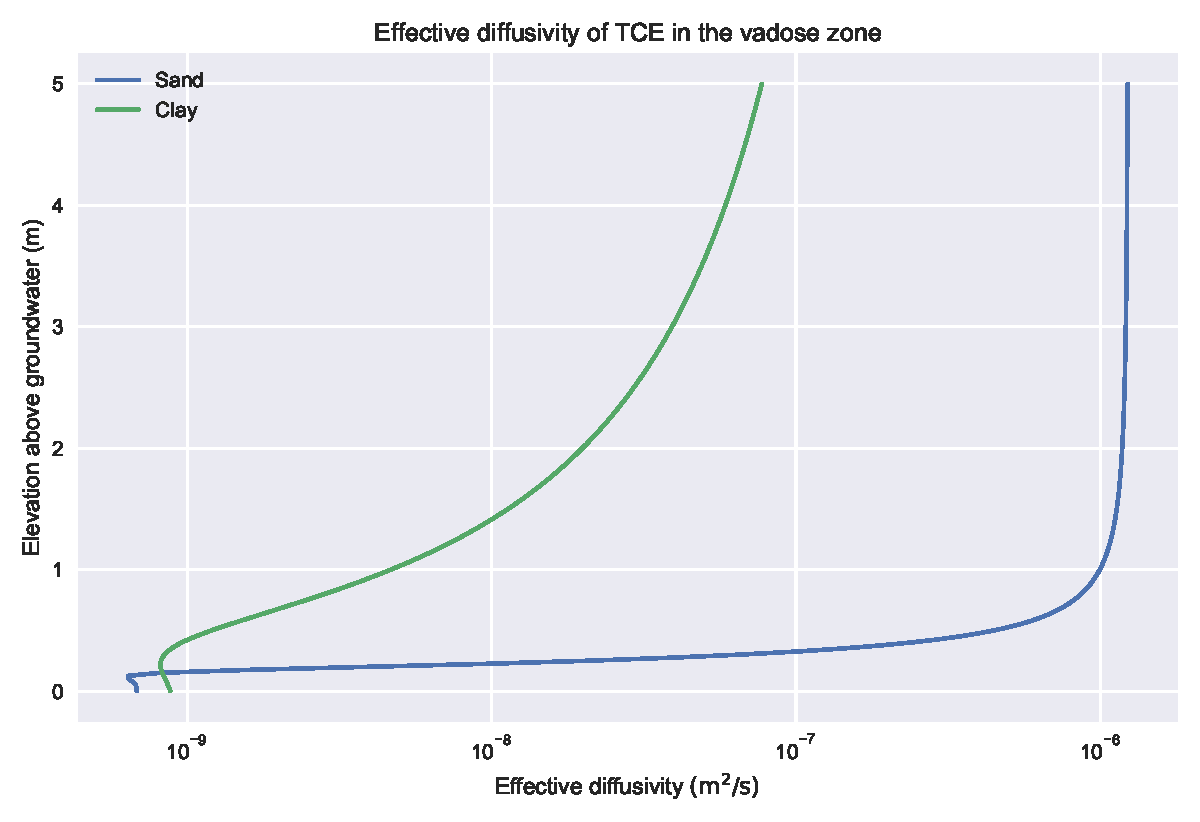
\includegraphics[width=0.75\textwidth]{effective_diffusivity.pdf}
  \caption[Effective diffusivity of TCE in the vadose zone.]{Effective diffusivity of TCE in the vadose zone using the Millington-Quirk model. Soil water and gas filled porosites are calculated using van Genuchten's equations.}
  \label{fig:D_eff}
\end{figure}

Putting all this together finally gives us the governing equation for contaminant transport in the vadose zone for our modeled VI scenario.
\begin{equation}\label{eq:mass_transport}
  R \frac{\partial c_w}{\partial t} = \nabla \cdot (D_\mathrm{eff} \nabla c_w) - K_H \vec{u}_g \cdot \nabla c_w
\end{equation}
To solve this we need to define some boundary and initial conditions.
We also need to choose a basis function which is used to determine the contaminant concentration throughout the domain, and we use the COMSOL recommended second order polynomial here.\par

\paragraph{Boundary Conditions}

In this VI scenario, the sole contaminant source is assumed to be the homogenously contaminated groundwater, which we assume to have a fixed concentration.
The atmosphere acts as a contaminant sink and thus this is simply a zero concentration boundary condition.
Contaminants leave the soil domain and enter the building through a combination of advective and diffusive gas phase transport.
The boundary condition applied to all other boundaries is a no-flow boundary.
\begin{align}
  &\text{Atmosphere} & c_w = \SI{0}{\mol\per\metre\cubed} \\
  &\text{Groundwater} & c_w = c_{gw} = \SI{50}{\micro\mol\per\metre\cubed} \\
  &\text{Foundation crack} & -\vec{n} \cdot \vec{N} = -j_{ck} \; \si{\mol\per\metre\squared\per\second}\\
  &\text{All other} & -\vec{n} \cdot \vec{N} = \SI{0}{\mol\per\metre\squared\per\second}
\end{align}
$\vec{n} \cdot \vec{N}$ is the dot product between the boundary normal vector and the contaminant flux;
$j_ck$ [\si{\mol\per\metre\squared\per\second}] is the contaminant flux into the building from section \ref{sec:indoor}.\par

\paragraph{Initial Conditions}

For steady-state problems, the initial conditions do not enter.
Transient simulations however, require initial conditions and these are assumed to be given by the steady-state solution.\par
